\section{Estado del arte}

% Estado del arte del tema en cuestión.
% Debería acabar mostrando por qué el trabajo es importante y aporta algo y con las hipótesis del trabajo.

Con anterioridad se han comentado algunas de las incursiones más antiguas en la generación de voz, destacando artefactos mecánicos, sistemas pneumáticos o sistemas de electrónica analógica. 

Ninguna de esas formas de síntesis de voz se emplea ya en la actualidad, por lo que no entraremos en detalles sobre ellos. Actualmente toda la síntesis de voz se realiza computacionalmente, pero no existe una única forma de abordar esta tarea por parte de un ordenador.

Haremos un repaso de la evolución de las diferentes soluciones para finalmente llegar a los modelos entrenados que mejores resultados ofrecen en la actualidad.

\subsection{Sistemas no entrenados}

Antes de que la investigación en inteligencia artificial y el avance de la tecnología permitiesen abordar muchos problemas mediante el entrenamiento de modelos, la mayoría de problemas complejos en el ámbito de la informática se intentaban resolver con un amplio conocimiento del dominio abordado.

Muchos de estos problemas además tenían la complejidad añadida de que eran multidiscipinares y requerían de un equipo de desarrollo especialmente docto en diferentes ámbitos y sus intersecciones. 
Incluso cumpliendo con estos requisitos humanos, muchos problemas no podían ser resueltos programáticamente por su dimensión o bien las soluciones que se les podía dar eran subóptimas. 

\subsubsection{MBROLA + eSpeak NG}

El proyecto MBROLA \hyperref[EA_1]{[5]} publicó su primera versión en 1995 como un proyecto del TCTS Lab de la Faculté Polytechnique de Mons. Su funcionamiento explota el uso de parejas de fonemas como unidad básica para la síntesis de voz junto a información prosódica. 
El proyecto se define actualmente de la siguiente forma:

«MBROLA is a speech synthesizer based on the concatenation of diphones. It takes a list of phonemes as input, together with prosodic information (duration of phonemes and a piecewise linear description of pitch), and produces speech samples on 16 bits (linear), at the sampling frequency of the diphone database.»

Pero MBROLA no se considera un sistema TTS completo, precisa de una primera conversión de texto a fonemas e información prosódica. Habitualmente el sistema se ha completado con eSpeak o su versión más moderna eSpeak NG, como primera etapa de recibe texto y lo convierte a una secuencia de fonemas.

Ambos componentes son software libre y el estándar de facto en muchos sistemas actuales de lectores de pantalla por su reducido tamaño y uso de recursos.

Aunque ni MBROLA ni eSpeak son herramientas entrenadas en forma alguna, se ha visto como eSpeak suele emplearse aún como un preprocesador de texto para alimentar a muchos modelos que se consideran entrenados end-to-end actualmente.

eSpeak permite no solamente convertir cualquier texto a una secuencia de fonemas en base a reglas definidas sino que también es capaz de resolver a fonemas otras expresiones habituales como cifras numéricas y símbolos\footnote{Ninguno de los modelos entrenados modernos puede asumir esta tarea por sí mismo, incluso si se le entrena con un dataset que incluya estos símbolos, pues la relación entre los símbolos y la secuencia de fonemas es demasiado compleja comparada con la que existe con el texto general}.


\subsection{Sistemas entrenados por componentes}

Aquí encontramos la primera incursión en la propuesta de un sistema totalmente entrenado, con anterioridad algunos sistemas han empleado algunos componentes entrenados de forma aislada pero seguían siendo predominantemente paramétricos.

\subsubsection{Deep Voice}

Deep Voice \hyperref[EA_4]{[6]} es un modelo desarrollado por el laboratorio de Inteligencia Artificial de Baidu. Se presentó a principios del año 2017 como el primer modelo donde todos sus componentes eran entrenados.

Este modelo tiene un total de cinco componentes fundamentales según sus autores explican:

\begin{itemize}
    \item Grafema a fonema: transforma los símbolos escritos a una representación fonética, en el caso del modelo solo se contempla el alfabeto inglés y la representación fonética ARPABET.
    \item Segmentación de sonido: dada una muestra de audio es capaz de identificar el comienzo y fin de cada fonema.
    \item Duración de fonemas: predice la duración de cada fonema dentro de una secuencia.
    \item Frecuencia fundamental: predice la forma en la que un fonema será pronunciado.
    \item Síntesis de audio: combina el resultado de los otros cuatro modelos
\end{itemize}

Aunque este modelo es el primero que no depende de otros componentes previos y es totalmente independiente en su funcionamiento de otros sistemas previos, su entrenamiento se realiza componente a componente y esto hace que el resultado final sea ligeramente pobre. 

\begin{center}
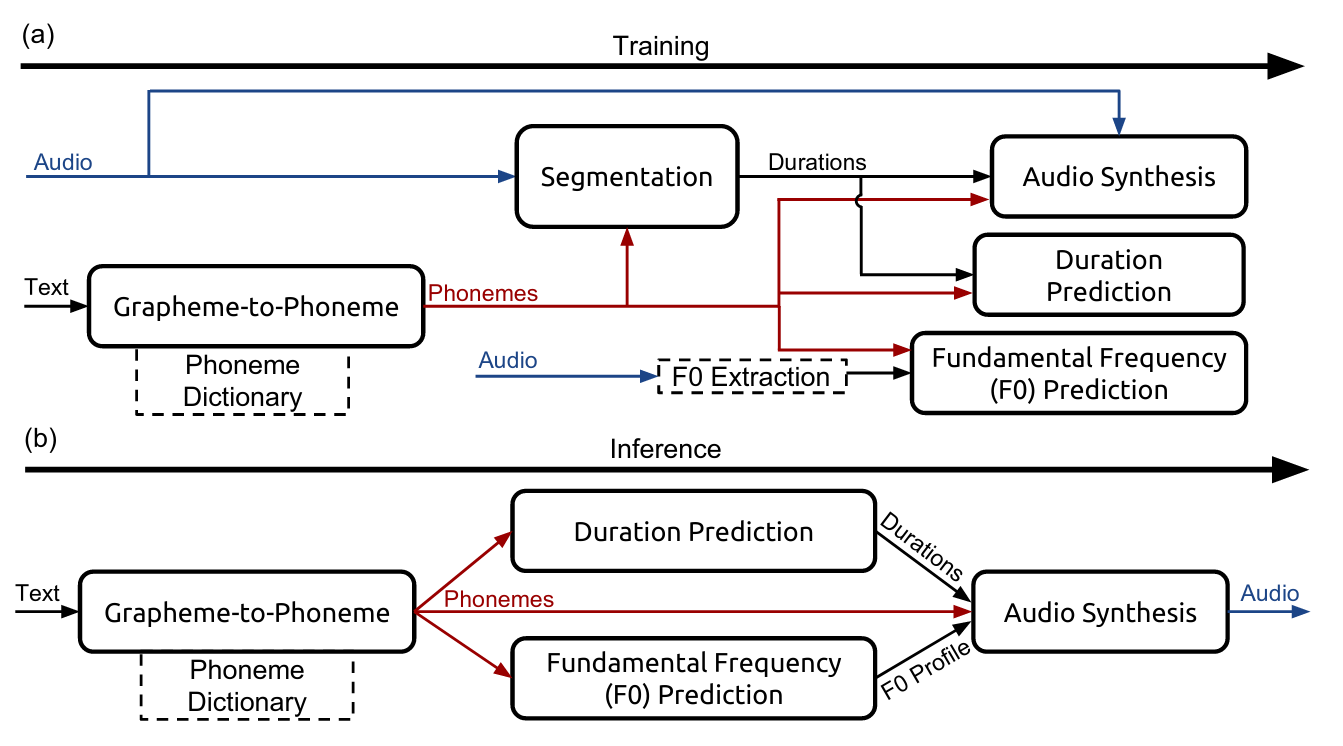
\includegraphics[width=14cm]{4_estado_del_arte_img/deepvoice_diagram.png}
\end{center}

En los modelos donde cada componente existe como una caja negra que solamente recibe una entrada y ofrece una salida, los errores se van acumulando en cascada sin que pueda existir una retroalimentación ni en la fase de entrenamiento ni en la fase de inferencia.

\subsection{Sistemas extremo a extremo bipartitos}

Estos sistemas reutilizan vocoders existentes también entrenados para ensamblarse como un sistema completo, pero su componente principal no podemos considerarlo un sistema de texto a voz completo sino un sistema de texto a espectrograma, siendo este espectrograma la entrada del vocoder.

Entre los vocoders habituales encontramos WaveNet, que ya se empleaba en el sistema mucho más modularizado de Deepvoice.

\subsubsection{Tacotron}

Poco después de la publicación del modelo Deep Voice, otro equipo de investigadores de Google publicaron el primer modelo \hyperref[EA_5]{[7]} que afirmaba ser un sistema TTS end-to-end: Tacotron.

Prácticamente a partir de este punto todos los autores afirman que su modelo funciona extremo a extremo, aunque dicha afirmación debe ser tomada con cautela. Es cierto que Tacotron tiene una arquitectura mucho más cohesionada que Deep Voice, donde la mayoría de componentes relevantes conforman un único modelo entrenado.

\begin{center}
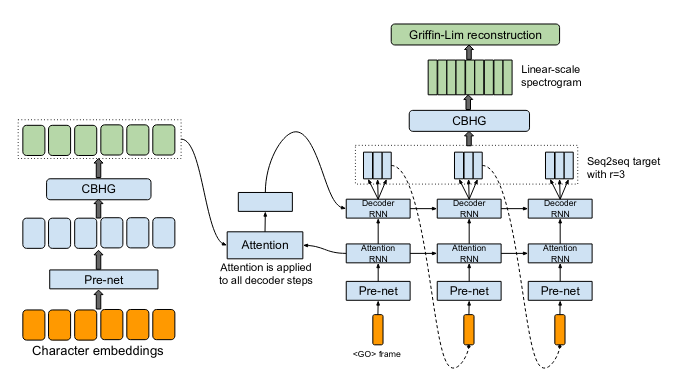
\includegraphics[width=14cm]{4_estado_del_arte_img/tacotron_0.png}
\end{center}

Pero la salida propiamente del modelo es un espectrograma y el componente final que transforma dicho espectrograma en una forma de onda no es entrenable. En la publicación original se dice:

\begin{displayquote}

«While Griffin-Lim is differentiable (it does not have trainable weights), we do not
impose any loss on it in this work. We emphasize that our choice of Griffin-Lim is for simplicity; while it already yields strong results, developing a fast and high-quality trainable spectrogram to waveform inverter is ongoing work.»

\end{displayquote}

Aún así, este modelo abrió la puerta a todos los desarrollos actuales basados en modelos cada vez más avanzados y aspirando cada vez más a incorporar más y más componentes para se efectivamente end-to-end.

Otra de las características significativas de este modelo es el uso de una arquitectura codificador-decodificador con un paradigma basado en atención. Esto supone que el modelo tiene una etapa intermedia donde la entrada de datos se codifica a una representación intermedia que luego se decodifica para generar el resultado deseado.

Esta etapa de compresión de datos además emplea un paradigma de atención, que en reglas generales supone el remarque de cierta información sobre otra en base a un criterio (temporal, espacial, etc...) para "atender" a lo más relevante a la hora de entrenar el modelo.

La representación adecuada de la información en estos estados internos para una efectiva comunicación entre en codificador y el decodificador es lo que entendemos por alineamiento en la etapa de entrenamiento y suele representarse con diagramas como este.

\begin{center}
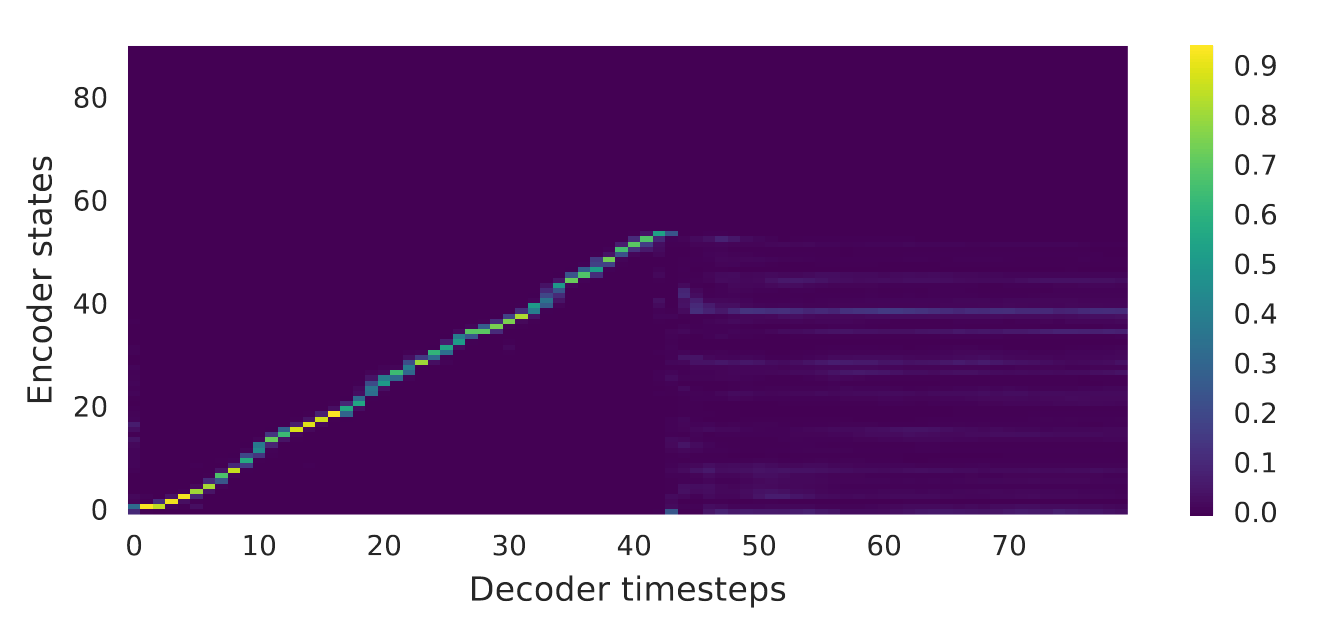
\includegraphics[width=14cm]{4_estado_del_arte_img/tacotron_1.png}
\end{center}

\subsubsection{Tacotron 2}

Del mismo equipo de ingenieros de Google llegó un año después de la publicación de Tacotron la siguiente iteración \hyperref[EA_6]{[8}, donde mejoran la arquitectura anterior y sobre todo abordan un mejor vocoder, uno de los puntos más flojos de Tacotron.

En este caso el vocoder pasa a ser un modelo entrenado llamado WaveNet  \hyperref[EA_7]{[9]}. Este modelo generativo de audio emplea un tipo de red RNN con convoluciones dilatadas que permiten reducir el número de capas ocultas y la cantidad de conexiones.

\begin{figure}[H]
\centering
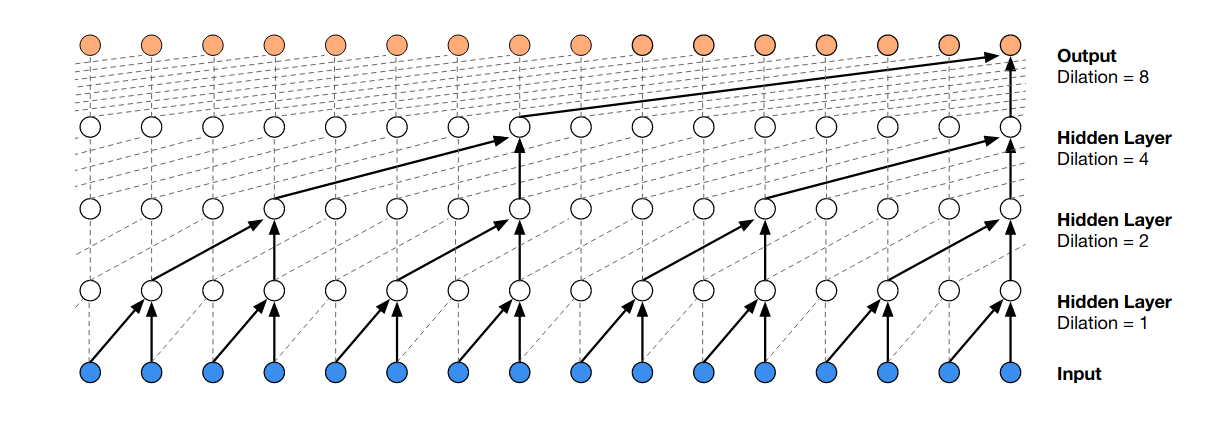
\includegraphics[width=14cm]{4_estado_del_arte_img/wavenet_0.png}
\caption{Diagrama del modelo WaveNet.}
\label{fig:figure1}
\end{figure}

Sus autores apuntan algo que más arriba habíamos mencionado ya, estos modelos precisan de poco o ningún conocimiento del dominio de la síntesis de voz para obtener resultados mejores que los modelos paramétricos que habían precisado una labor inmensa de ingeniería de características.

\begin{displayquote}
«The resulting system synthesizes speech with Tacotron-level prosody and WaveNet-level audio quality. This system can be trained directly from data without relying on complex feature engineering, and achieves state-of-the-art sound quality close to that of natural human speech.»
\end{displayquote}

Por lo demás Tacotron 2 conserva las características fundamentales de la arquitectura de Tacotron pero la incorporación de un vocoder mejor supone una mejora notable de la calidad de audio final. 


\begin{figure}[H]
\centering
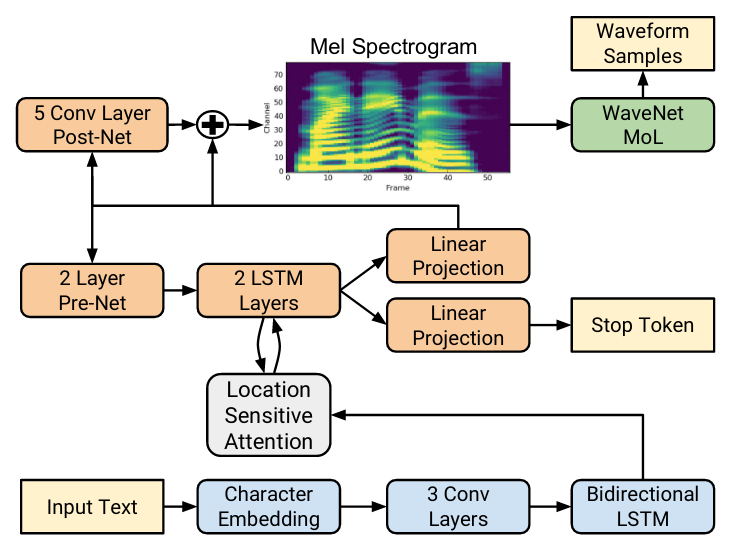
\includegraphics[width=12cm]{4_estado_del_arte_img/tacotron2_0.png}
\caption{Diagrama del modelo Tacotron 2.}
\label{fig:figure1}
\end{figure}


\subsection{Sistemas extremo a extremo monolíticos}

Se trata de sistemas completamente extremo a extremo, sin tener componentes desarrollados de forma independiente como el caso de Tacotron y Tacotron 2. Esto no significa que no puedan identificarse diferentes elementos o componentes en el modelo, lo que significa es que estos componentes están estrechamente relacionados y se pueden entrenar como uno solo.

\subsubsection{VITS}

Este es el modelo presentado a mediados de 2021 supone un gran salto frente a modelos anteriores basados en dos componentes conectados mediante una representación de características lingüísticas o bien un espectrograma tipo MEL.

VITS (Variational Inference with adversarial learning for end-to-end Text-to-Speech)  \hyperref[EA_8]{[10]} presenta un sistema realmente end-to-end que consigue dar solución a la dificultad de entrenar modelos donde se encadenan muchos elementos en cascada. 

Otros modelos antes que VITS intentaron hacer una propuesta de un sistema completo, extremo a extremo, pero la falta de paralelización en sus propuestas suponía un problema de rendimiento importante. Este podría ser el caso de Transformer TTS, que intentó adaptar un modelo de gran éxito en otros ámbitos NLP.

La arquitectura de VITS integra en un mismo modelo también el vocoder responsable de la generación final de sonido, además de otras características como un generador estocástico que permite a partir de una misma entrada generar resultados distintos.


\begin{figure}[H]
\centering
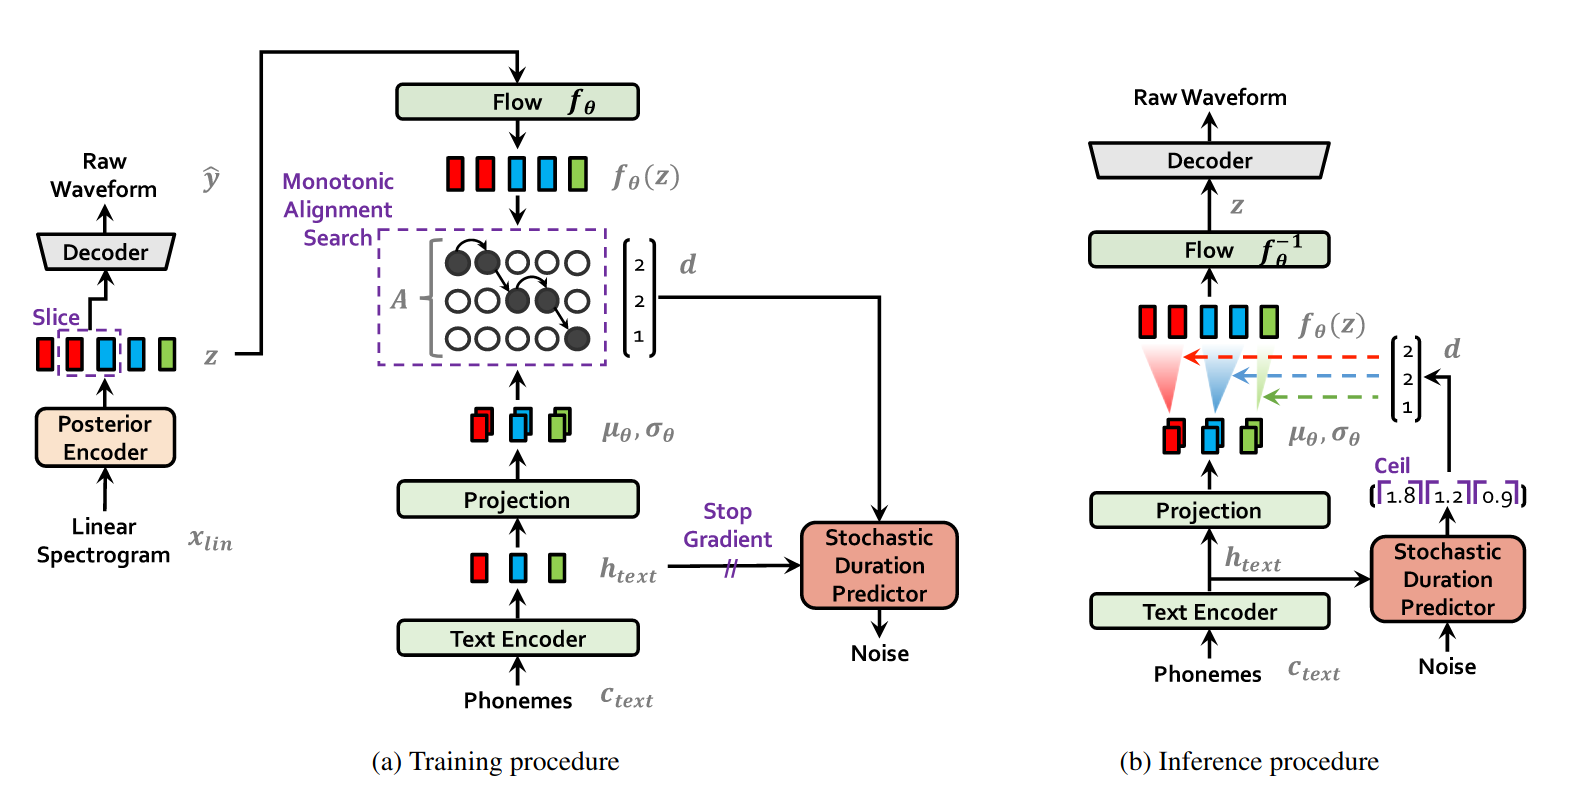
\includegraphics[width=14cm]{4_estado_del_arte_img/vits_0.png}
\caption{Diagrama del modelo VITS.}
\label{fig:figure1}
\end{figure}


VITS también permite entrenar simultáneamente un conjunto de hablantes distintos para obtener un único modelo final que permitirá seleccionar el hablante sobre el que realizar la inferencia. 

El motivo por el cual el entrenamiento de modelos en general requiere de unidades de procesamiento que explotan el paralelismo masivo como las GPUs o que además tienen hardware especialmente diseñado como las TPU o NPU, es porque no existe otra forma de acelerar la ingente cantidad de cálculos que requiere esta tarea.

Un modelo que no tenga posibilidades de ser paralelizado no es un modelo viable en la actualidad, por eso este modelo a efectos prácticos y probables representa el estado del arte en la síntesis de voz a partir de texto.

\subsection{Sistemas con características adicionales}

Hasta el momento hemos visto únicamente modelos que parten de cero, es decir, que son entrenados mayormente sobre un dataset particular y ofrecerán inferencias con lo aprendido al haber sido entrenados sobre dicho dataset.

Algunos desarrolladores han experimentado continuando el entrenamiento anterior sobre un dataset nuevo con la idea de conseguir una voz particular sobre un dataset mucho mayor con una voz distinta, pero los resultados de esto son dispares y no se han encontrado publicaciones serias al respecto. 

Esta forma de trabajar es lo que se denomina transferencia de aprendizaje, una técnica empleada en otros ámbitos del Aprendizaje Computacional.

\subsubsection{YourTTS}

Hace apenas unos meses se publicó este nuevo modelo  \hyperref[EA_9]{[11]} que se construye sobre la arquitectura base de VITS y aspira a permitir realizar una adaptación a un hablante nuevo en la etapa de inferencia y no en el propio entrenamiento.

Este modelo da un paso más allá y nos acerca en gran medida a tender puentes realistas hacia la generación de deepfakes sin grandes conocimientos técnicos ni gran esfuerzo\footnote{Esto es algo que preocupa a los autores de esta publicación, tanto es así que públicamente rechazan en estos momentos dar consejos ni detalles sobre ajustes finos del modelo para gente fuera de la comunidad investigadora. \url{https://github.com/Edresson/YourTTS/issues/5}}.

Por desgracia lo prometedor de este modelo no es algo que hayamos podido explotar en este trabajo, al depender sus resultados de un entrenamiento bastante amplio de VITS con múltiples hablantes, cosa que a día de hoy no existe en castellano.

Los autores de esta publicación afirman que con una muestra de menos de un minuto de voz se puede conseguir un clonado aceptable:

\begin{displayquote}
«Require less than 1 minute of speech to fine-tune the model for speakers who have voice/recording characteristics very different from those seen in model training, and still achieve good similarity and quality results»
\end{displayquote}

Aún sin haber podido probar lo cierto o falso de dicha afirmación, otras afirmaciones previas en este ámbito han probado tener una tendencia a la hipérbole y a centrar la atención en los casos ideales y no en los resultados habituales.

\subsection{Toolkits}

La proliferación de numerosos modelos y variaciones de los mismos presenta un reto a la hora de pasar de la investigación académica a la implementación de sistemas reales en producción. 

Muchos de los modelos arriba comentados además no siempre se acompañan con una implementación de referencia, o dicha implementación ha quedado tan obsoleta que otras implementaciones alternativas se vuelven la referencia de facto.

En esta situación se han constituido diversos toolkits que intentan encapsular muchos de estos modelos o componentes en un formato más accesible al integrador de sistemas o al usuario final. El ámbito de estos toolkits además no suele limitarse a los modelos de texto a voz en los que nos hemos centrado sino a otros ámbitos como el reconocimiento automático del habla.

\subsubsection{ESPnet}

El proyecto ESPnet  \hyperref[EA_2]{[12]} se define a sí mismo como:

\begin{displayquote}
«ESPnet is an end-to-end speech processing toolkit covering end-to-end speech recognition, text-to-speech, speech translation, speech enhancement, speaker diarization, spoken language understanding, and so on»
\end{displayquote}

Su objetivo es recopilar diferentes componentes para el procesamiento natural del lenguaje orientado a la síntesis de voz y la interpretación de la voz con el fin de crear un ecosistema que haga compatibles todos estos elementos e implementaciones.

Muchos de los modelos que hemos comentado anteriormente está integrados en ESPnet y hacer uso de ellos resulta así más sencillo y en cierto grado estandarizado.

\subsubsection{Coqui-AI}

De manera similar a ESPnet, Coqui-AI  \hyperref[EA_3]{[13]} es otro proyecto que aspira a generar un ecosistema que integre muchos de los desarrollos más actuales en el reconocimiento automático del habla así como en la síntesis de voz.

A diferencia de ESPnet, Coqui-AI tiene proyectos separados para los modelos TTS y los modelos ASR, por lo que el ecosistema es algo más pequeño y permite una curva de aprendizaje menos abrupta. En sus propios términos el proyecto afirma:

\begin{displayquote}
«TTS is a library for advanced Text-to-Speech generation. It's built on the latest research, was designed to achieve the best trade-off among ease-of-training, speed and quality»
\end{displayquote}

Este toolkit fue el que se decidió emplear para facilitar los entrenamientos de los modelos que finalmente se decidiesen entrenar. Hay dos grandes ventajas del uso de un entorno de este tipo: por una parte la base de código de los modelos ha sido mejor revisado y mantenido; por otra parte poder reutilizar herramientas para el entrenamiento como las necesarias para preparar el dataset reduce la cantidad de trabajo técnico específico para cada dataset.

\subsection{Conclusiones}

El estudio del Estado del Arte nos pone en situación de comprender el máximo punto de desarrollo de la investigación en el dominio que hemos definido para este trabajo, ahora conocemos no solo los modelos más avanzados para la generación de voz de forma sintética sino también algunos ecosistemas de herramientas que nos facilitarán dar pasos en la dirección de estudio que apuntaba la introducción de este proyecto de investigación. 

\newpage 